%
% LSST Data Products Definition Document
%
% Maintained by Mario Juric <mjuric@lsst.org>
%
\documentclass[12pt]{article}

\usepackage[english]{babel}
\usepackage[utf8x]{inputenc}
\usepackage{amsmath}
\usepackage{graphicx}
\usepackage{longtable}
\usepackage{hyperref}
\usepackage{comment}
\usepackage{float}

\excludecomment{changelog}

\newcommand\x         {\hbox{$\times$}}
\newcommand\othername {\hbox{$\dots$}}
\def\eq#1{\begin{equation} #1 \end{equation}}
\def\eqarray#1{\begin{eqnarray} #1 \end{eqnarray}}
\def\eqarraylet#1{\begin{mathletters}\begin{eqnarray} #1 
                  \end{eqnarray}\end{mathletters}}
\def\mic              {\hbox{$\mu{\rm m}$}}
\def\about            {\hbox{$\sim$}}
\def\Mo               {\hbox{$M_{\odot}$}}
\def\Lo               {\hbox{$L_{\odot}$}}
\def\comm#1           {{\tt (COMMENT: #1)}}
\def\kms   {\hbox{km s$^{-1}$}}

\usepackage[usenames]{color} 
\newcommand{\G}[1]{{\color{red} #1}}
\newcommand{\B}[1]{{#1}}
\newcommand{\R}[1]{{\color{red}}}
\newcommand{\code}[1]{\texttt{#1}}

\usepackage{xspace}
\newcommand{\DIASource}{\code{DIASource}\xspace}
\newcommand{\DIASources}{\code{DIASources}\xspace}
\newcommand{\DIAObject}{\code{DIAObject}\xspace}
\newcommand{\DIAObjects}{\code{DIAObjects}\xspace}
\newcommand{\DB}{{Level 1 database}\xspace}
\newcommand{\DR}{{Level 2 database}\xspace}
\newcommand{\Object}{\code{Object}\xspace}
\newcommand{\Objects}{\code{Objects}\xspace}
\newcommand{\Source}{\code{Source}\xspace}
\newcommand{\Sources}{\code{Sources}\xspace}
\newcommand{\ForcedSource}{\code{ForcedSource}\xspace}
\newcommand{\ForcedSources}{\code{ForcedSources}\xspace}
\newcommand{\SSObject}{\code{SSObject}\xspace}
\newcommand{\SSObjects}{\code{SSObjects}\xspace}
\newcommand{\VOEvent}{\code{VOEvent}\xspace}
\newcommand{\VOEvents}{\code{VOEvents}\xspace}

\title{Large Synoptic Survey Telescope \\
Data Products Definition Document \\
(*** DRAFT ***)}
\author{
    Mario Juri\'c \textless\href{mailto:mjuric@lsst.org}{mjuric@lsst.org}\textgreater \vspace{1ex} \\
    {\em with input from} \vspace{1ex} \\
    T. Axelrod, A.C. Becker, J. Becla,  G.P. Dubois-Felsmann, \\
    M. Freemon, \v{Z}. Ivezi\'c, J. Kantor, K-T Lim, R. Lupton, \\
    D. Shaw, M. Strauss, {\em and} J.A. Tyson \vspace{1.2ex} \\
    {\em for the LSST Project}
}

\begin{document}
\maketitle

\begin{abstract}
This document describes the plans for contents of Level 1 and 2 LSST data
products, and the rationale behind various choices that were made. This is an
{\bf internal draft} and a work in progress. {\bf It should not be circulated
widely until this notice is removed.}
\end{abstract}

\tableofcontents

\section{Introduction}

% Note: paragraph lifted from Zeljko's overview paper
LSST will be a large, wide-field ground-based optical telescope system
designed to obtain multiple images covering the sky that is visible from Cerro
Pach\'{o}n in Northern Chile. The current baseline design, with an 8.4m (6.7m
effective) primary mirror, a 9.6 deg$^2$ field of view, and a 3.2 Gigapixel
camera, will allow about 10,000 square degrees of sky to be covered using
pairs of 15-second exposures \R{in two photometric bands} \B{twice per night}
every three nights on average, with typical 5$\sigma$ depth for point sources
of $r\sim24.5$ (AB). The system is designed to yield high image quality as
well as superb astrometric and photometric accuracy. The \B{total} survey area
will include 30,000 deg$^2$ with $\delta<+34.5^\circ$, and will be imaged
multiple times in six bands, $ugrizy$, covering the wavelength range 320--1050
nm. The project is scheduled to begin the regular survey operations at the
start of next decade. About 90\% of the observing time will be devoted to a
deep-wide-fast survey mode which will \B{uniformly} observe a 18,000 deg$^2$
region about 1000 times (summed over all six bands) during the anticipated 10
years of operations, and yield a coadded map to $r\sim27.5$. These data will
result in databases including 10 billion galaxies and a similar number of
stars, and will serve the majority of the primary science programs. The
remaining 10\% of the observing time will be allocated to special projects
such as a Very Deep and Fast time domain survey.

The LSST will be operated in fully automated survey mode. The images acquired
by the LSST Camera will be processed by LSST Data Management software to a)
detect and characterize imaged astrophysical sources and b) detect and
characterize changes in time in LSST-observed universe. The results of that
processing will be reduced images, catalogs of detected objects and the
measurements of their properties, and prompt alerts to ``events'' -- changes
in astrophysical scenery discovered by differencing incoming images against
older, deeper, images of the sky in the same direction ({\em templates}, see
\S \ref{sec:templates}).

\vspace{1em}

The {\em broad}, {\em high-level}, requirements for LSST Data Products are
given by the LSST Science Requirements Document. This document lays out the
{\em specifics} of what the data products will comprise of, how those data
will be generated, and when. It serves to inform the flow-down from the {\em
LSST Science Requirements Document} and the {\em LSST Observatory System
Specifications}, to the {\em LSST Data Management System Requirements}
document, the UML model, and the database schema.

\subsection{Level 1 and 2 Data Products}

LSST Data Management will perform two, somewhat overlapping in scientific
intent, types of image analyses:

\begin{enumerate}
\item Analysis of difference images, with the goal of detecting and
      characterizing astrophysical phenomena revealed by their time-dependent
      nature. The detection of supernovae superimposed on bright extended
      galaxies is an example of this analysis. The processing is done on a
      nightly or daily basis and produces {\bf Level 1} data products. They
      include the difference images, the sources detected in difference images
      (\DIASources), astrophysical objects\footnote{The LSST has adopted the
      nomenclature by which single-epoch detections of astrophysical {\em
      objects} are called {\em sources}. This nomenclature is not universal:
      some surveys call {\em detections} what we call {\em sources}, and use
      the term {\em sources} for what we call {\em objects}.} these are
      associated to (\DIAObjects), and Solar System objects
      (\SSObjects\footnote{\SSObjects used to be called call ``Moving
      Objects'' in previous versions of the Data Products baseline. The name
      is potentially confusing as high-proper motion stars are moving objects
      as well. A more accurate distinction is the one between objects inside
      and outside of the Solar System.}). These are added to the {\bf \DB} and
      made available in real time. Notifications (``alerts'') about new
      \DIASources will be issued using community-accepted standards within 60
      seconds of observation.
\item Analysis of direct images, with the goal of detecting and characterizing
      astrophysical objects. Detection of faint galaxies on deep co-adds and
      their subsequent characterization is an example of this analysis. The
      results are {\bf Level 2} data products. These products, released
      annually\footnote{Except for the first two data releases, which will be
      created six months apart.}, will include the single-epoch images, deep
      co-adds, catalogs of \Objects (detections on deep co-adds) and
      \Sources\footnote{When written in bold monospace type, \Objects and
      \Sources refer to objects and sources detected and measured as a part of
      Level 2 processing.} (measurements on individual direct images), as well
      as fully reprocessed Level 1 data products (see \S
      \ref{sec:l1dbreproc}). In contrast to the \DB, which is updated in
      real-time, the \DR{}s are static and will not change after release.
\end{enumerate}
 
The two types of analyses have different requirements on timeliness. Changes
in flux or position of objects may need to be immediately followed up, lest
interesting information be lost. Thus the primary results of analysis of
difference images -- discovered and characterized \DIASources{} -- generally
need to be broadcast as {\em event alerts} within 60 seconds of end of
visit\footnote{The LSST takes two (nominally 15 second) exposures per
pointing, called {\em snaps}. That pair of exposures is called a {\em visit}.}
acquisition. The analysis of science (direct) images is less time sensitive,
and will be done as a part of annual data release process.

%In both cases, the software analyzes the image data to detect {\em sources},
%groupings of pixels with values inconsistent with being noise at some preset
%level (eg., a typical threshold is $S/N = 5$). If the detection is performed
%on science images, we call the resulting sources {\em Sources}\footnote{Note
%the capitalization}. If the source has been detected on a difference image, we
%call it a {\em DIASource}\footnote{for {\em Difference Image Analysis
%Source}}.

%Once detected, the sources can be associated to {\em Objects}, and be
%characterized in various ways (eg., by PSF flux measurement, model fitting,
%shape measurement, etc.).

\section{Level 1 Data Products}

\subsection{Overview}

Level 1 data products are a result of difference image analysis (DIA; \S
\ref{sec:dia}). They include the sources detected in difference images
(\DIASources), astrophysical objects that these are associated to
(\DIAObjects), identified Solar System objects\footnote{The LSST SRD considers
Solar System object orbit catalog to be a Level 2 data product (LSSTSRD, Sec
3.5). Nevertheless, to successfully differentiate between apparitions of known
Solar System objects and other types \DIASources we consider it functionally a
part of Level 1.} (\SSObject), and related, broadly defined, metadata
(including eg., cut-outs\footnote{Small, $30 \times 30$, sub-images at the
position of a detected source. Also known as {\em postage stamps.}}).

\DIASources are sources detected on difference images (those above $S/N=5$
after correlation with an appropriate PSF profile). They represent changes in
flux with respect to a deep template. Physically, a \DIASource may be an
observation of new astrophysical object that was not present at that position
in the template image (for example, an asteroid), or an observation of flux
change in an existing source (for example, a variable star). Their flux can be
negative (eg., if a source present in the template image reduced its
brightness, or moved away).

Groups of \DIASources detected on visits taken at different times are
associated with either a \DIAObject or an \SSObject to represent the
underlying astrophysical phenomenon. The association can be made in two
different ways: by assuming the underlying phenomenon is an object within the
Solar System moving on an orbit around the Sun\footnote{We don't plan to fit
for motion around other Solar System bodies; eg., identifying new satellites
of Jupiter is left to the community.}, or by assuming it to be distant enough
to only exhibit small parallactic and proper motion\footnote{Where 'small' is
small enough to unambiguously positionally associate together individual
apparitions of the object.}. The latter type of association is performed
during difference image analysis right after the image has been acquired. The
former is done at daytime by the Moving Objects Processing Software
(\code{MOPS}), unless the \DIASource is an apparition of an already known
\SSObject. In that case, it will be flagged as such during difference image
analysis.

All \DIASources will be alerted on at the end of the difference image
analysis\footnote{For observations on the ecliptic near the opposition, Solar
System objects will dominate the \DIASource counts, and (until they're
recognized as such) overwhelm the explosive transient signal. It will
therefore be advantageous to quickly identify the majority of Solar System
objects early in the survey.}.

\subsection{Level 1 Data Processing}

\subsubsection{Difference Image Analysis}
\label{sec:dia}

The following is a high-level description of steps which will occur during
regular difference image analysis:
%
\begin{enumerate}
\item A visit is acquired and reduced to a single {\em visit image} (cosmic
      ray rejection, instrumental signature removal\footnote{Eg., subtraction
      of bias and dark frames, flat fielding, bad pixel/column interpolation,
      etc.}, combining of snaps}, etc.).
\item The visit image is differenced against the appropriate template and
      \DIASources are detected.
\item The flux and shape\footnote{The ``shape'' in this context are weighted
      2$^{\rm nd}$ moments, as well as a fit to a trailed source model.} of
      the DIASource are measured on the difference image. The visit image is
      force-photometered at the position of the \DIASource to obtain a measure
      of the absolute flux. No deblending will be attempted.
\item The \DB (see \S \ref{sec:level1db}) is searched for a \DIAObject or
      \SSObject with which to positionally associate the observed
      \DIASource\footnote{The association algorithm will guarantee that a
      \DIASource is associated with not more than one \DIAObject or \SSObject.
      The algorithm will take into account the parallax and proper or
      Keplerian motions, as well as the errors in estimated positions of
      \DIAObject, \SSObject, and \DIASource to find the maximally likely
      match. Multiple \DIASources in the same visit will not be matched to the
      same \DIAObject.}. If no match is found, a new \DIAObject is created and
      the observed \DIASource is associated to it.
\item If the \DIASource has been associated with an \SSObject (a known Solar
      System object), it will be flagged as such and an alert will be issued.
      Further processing will occur in daytime (see section
      \ref{sec:ssProcessing}).
\item Otherwise, the associated \DIAObject measurements will be updated with
      new data. All affected columns will be recomputed, including proper
      motions, centroids, light curves, etc.
\item The \DR\footnote{\DR is a database resulting from annual data release
      processing.} is searched for one or more \Objects positionally close to
      the \DIAObject, out to some maximum radius\footnote{Eg., a few
      arcseconds.}. The IDs of these \Objects are recorded in the \DIAObject
      record and provided in the event alert.
\item An alert is issued that includes: the name of the \DB, the timestamp of
      when this database has been queried to issue this alert, the \DIASource
      ID, the \DIAObject ID\footnote{We guarantee that a receiver will always
      be able to regenerate the alert contents at any later date using the
      included timestamps and metadata (IDs and database names).}, name of the
      \DR and the IDs of nearby \Objects, and the associated science content
      (centroid, fluxes, low-order lightcurve moments, periods, etc.), {\em
      including the full light curves}. See Section \ref{sec:voEventContents}
      for a more complete enumeration.
\item For all \DIAObjects overlapping the field of view, to which a \DIASource
      from this visit has not been associated, forced photometry will be
      performed (point source photometry only). Those measurements will be
      stored as appropriately flagged \DIASources\footnote{For the purposes of
      this document, we're treating the \DIASources generated by precovery
      measurements to be the same as \DIASources detected in difference images
      (but flagged appropriately). In the logical schema, these may be divided
      into two separate tables.}. No alerts will be issued for these
      \DIASources.
\item Within 24 hours of discovery, {\em precovery} PSF forced photometry will
      be performed on any difference image overlapping the position of new
      \DIAObjects taken within the past 30 days, and added to the database.
      Alerts will not be issued with precovery photometry information.

\end{enumerate}

In addition to the processing described above, a smaller sample of sources
detected on difference images {\em below} the nominal $S/N=5$ threshold will
be measured and stores, in order to enable monitoring of difference image
analysis quality.

Also, the system will have the ability to measure and alert on a
limited\footnote{It will be sized for no less than $\sim 10\%$ of average
\DIASource per visit rate.} number of sources detected below the nominal
threshold for which additional criteria are satisfied. For example, a $S/N =
3$ source detection near a gravitational keyhole may be highly significant in
assessing the danger posed by a potentially hazadous asteroid. The project
will define the initial set of criteria by the start of Operations.

\subsubsection{Solar System Object Processing}
\label{sec:ssProcessing}

The following will occur during regular Solar System object processing (in
daytime\footnote{Note that there {\em is no guarantee on when daytime Solar
System processing must finish}, just that, averaged over some reasonable
timescale (eg., a month), a night's worth of observing is processed within 24
hours. Nights rich in moving objects may take longer to process, while nights
with less will finish more quickly. In other words, the requirement is on {\em
throughput}, not latency.}, after a night of observing):
%
\begin{enumerate}
\item The orbits/physical properties of \SSObjects that were re-observed on
      the previous night are recomputed. Updated data are entered to the
      \SSObjects table.
\item All \DIASources detected on the previous night, that have not been
      matched with high probability to a known \Object, \SSObject, or an
      artifact, are analyzed for potential pairs, forming {\em tracklets}.
\item The collection of tracklets collected over the past 30 days is searched
      for subsets forming {\em tracks} consistent with being on the same
      Keplerian orbit around the Sun.
\item For those that are, an orbit is fitted and a new \SSObject table entry
      created. \DIASource records are updated to point to the new \SSObject
      record. \DIAObjects ``orphaned'' by this unlinking are
      deleted.\footnote{Some \DIAObjects may only be left with forced
      photometry measurements at their location (since all \DIAObjects are
      force-photometered on previous and subsequent visits); these will be
      kept but flagged as such.}.
\item Precovery linking is attempted for all \SSObjects whose orbits were
      updated in this process. Where successful, \SSObjects (orbits) are
      updated as needed.
\end{enumerate}

\subsection{The \DB}
\label{sec:level1db}

The described alert processing design presupposes the existence of a \DB that
contains the objects and sources detected on difference images. At the very
least\footnote{It will also contain exposure and visit metadata, MOPS-specific
tables, etc. These are either standard/uncontroversial, or
implementation-dependent, irrelevant for science, and therefore not discussed
here.}, this database will have tables of \DIASources, \DIAObjects, and
\SSObjects, populated in the course of difference image and Solar System
object processing\footnote{The latter is also colloquially known as {\em
DayMOPS}.}. As these get updated and added to, their updated contents becomes
visible (queryable) immediately\footnote{No later than the moment of issuance
of any event alert that may refer to it.}.

Note that {\em this database is only loosely coupled to the \DR}. All of the
coupling is through providing positional matches between the \DIAObjects
entries in the \DB and the \Objects in the \DR database. There is no direct
\DIASource-to-\Object match. The adopted data model emphasizes that {\em
having a \DIASource be positionally coincident with an \Object does not imply
it is physically related to it}. Absent other information, the least
presumptuous data model relationship is one of {\em positional association},
not {\em physical identity}.

This may seem odd at first: for example, in a simple case of a variable star,
matching individual \DIASources to \Objects is exactly what an astronomer
would want. That approach, however, fails in the following scenarios:
\begin{itemize}
\item {\em A supernova in a galaxy.} The matched object in the \Object table
      will be the galaxy, which is a distinct astrophysical object. We want to
      keep the information related to the supernova (eg., colors, the light
      curve) separate from those measurements for the galaxy.
\item {\em An asteroid occulting a star.} If associated with the star on first
      apparition, the association would need to be dissolved when the source
      is recognized as an asteroid (perhaps even as early as a day later).
\item {\em A supernova on top of a pair of blended galaxies.} It is not clear
      in general to which galaxy this \DIASource would belong. That in itself
      is a research question.
\end{itemize}

\vspace{1ex}

\DIASource-to-\Object matches can still be emulated via a three-step link
(\DIASource-\DIAObject-\Object). For ease of use, views or pre-built table
with these will be offered to end-users.

%There are three ``core'' tables in the \DB: the \DIASource table, with
%information about detected and/or measured \DIASources, \DIAObject table, with
%summary information about \DIAObjects derived from the associated \DIASources,
%and the \SSObject table (short for {\bf Solar System Object}\footnote{This is
%what we used to call a ``Moving Object''. This name is potentially confusing,
%as high-proper motion stars are moving objects as well. A more accurate
%distinction is the one between objects in an out of the Solar System.})
%holding derived orbits and associated Solar System Object-specific
%information.

\vspace{2em}

In the sections to follow, we present the {\em conceptual schemas} for the
most important \DB tables. These convey {\em what} data will be recorded in
each table, rather than the details of {\em how}. For example, columns whose
type is an array (eg., \texttt{radec}) may be expanded to one table column per
element of the array (eg., \texttt{ra}, \texttt{decl}) once this schema is
translated to SQL. Secondly, the tables to be presented are normalizes (i.e.,
contain no redundant information). For example, since the band of observation
can be found by joining a \DIASource table to the table with exposure
metadata, there's no column for 'band' in the \DIASource table. In the
as-built database, the views presented to the users will be appropriately
denormalized for ease of use.

\subsubsection{\DIASource Table}

This is a table of sources detected at $SNR \geq 5$ on difference images
(\DIASources). On average, we expect $\sim 2000$ \DIASources per visit ($\sim
2{\rm M}$ per night; 20,000 per deg$^2$ per hour).

Some $SNR \geq 5$ sources will not be caused by observed astrophysical
phenomena, but by artifacts (bad columns, diffraction spikes, etc.). The
difference image analysis software will attempt to identify and flag these as
such.

Unless noted otherwise, all \DIASource quantities (fluxes, centroids, etc.)
are measured on the difference image.

\begin{center}
\begin{longtable}{p{3cm}p{2cm}p{2cm}p{5cm}}
\caption[\DIASource Table]{\DIASource Table} \\

\hline \multicolumn{1}{c}{\bf Name} & \multicolumn{1}{c}{\bf Type} & \multicolumn{1}{c}{\bf Unit} & \multicolumn{1}{c}{\bf Description} \\ \hline
\endhead

\hline \multicolumn{4}{r}{{\em Continued on next page}} \\
\endfoot

\hline\hline
\endlastfoot

diaSourceId & uint128 & ~ & Unique source identifier \\ 

ccdVisitId & uint64 & ~ & Id. of CCD and visit where this source was measured \\ 

diaObjectId & uint128 & ~ & Id. of the \DIAObject this source was associated
with, if any. \\ 

ssObjectId & uint64 & ~ & Id. of the \SSObject this source has been linked to,
if any. \\ 

midPointTai & double & time & Time of mid-exposure for this DIASource. \\ 

radec & double[2] & degrees & $(\alpha, \delta)$\footnote{The astrometric
reference frame will be chosen closer to start of operations.} \\ 

radecCov & float[3] & various & \texttt{radec} covariance matrix \\ 

xy & float[2] & pixels & Column and row of the centroid. \\ 

xyCov & float[3] & various & Centroid covariance matrix \\ 

SNR & float & ~ & The signal-to-noise ratio at which this source was detected
in the difference image.\footnote{This is not necessarily the same as
psFlux/psFluxSigma, as the flux measurement algorithm may be more accurate
than the detection algorithm.} \\

psFlux & float & nmgy\footnote{A ``maggie'', as introduced by SDSS, is a
linear measure of flux; one maggie has an AB magnitude of 0. ``nmgy'' is short
for a nanomaggie. Flux of $0.063$~nmgy corresponds to a $24.5^{\rm th}$
magnitude star. See \S \ref{sec:fluxes} for details.} & Calibrated flux for
point source model. Note this actually measures the flux {\em difference}
between the template and the visit image. \\ 

psFluxSigma & float & nmgy & Estimated uncertainty of \texttt{psFlux}. \\

psLnL & float & ~ & Natural $log$ likelihood of the observed data given the
point source model. \\ 

trailFlux & float & nmgy & Calibrated flux for a trailed source
model\footnote{A {\em Trailed Source Model} attempts to fit a (PSF-convolved)
model of a point source that was trailed by a certain amount in some direction
(taking into account the two-snap nature of the visit, which may lead to a dip
in flux around the mid-point of the trail). Roughly, it's a fit to a
PSF-convolved line. The primary use case is to characterize fast-moving Solar
System objects.}$^,$\footnote{This model does not fit for the {\em direction}
of motion; to recover it, we would need to fit the model to separately to
individual snaps of a visit. This adds to system complexity, and is not
clearly justified by increased MOPS performance given the added information.}.
Note this actually measures the flux {\em difference} between the template and
the visit image. \\ 

trailLength & float & arcsec & Maximum likelihood fit of trail
length\footnote{Note that we'll likely measure trailRow and trailCol, and
transform to trailLength/trailAngle (or trailRa/trailDec) for storage in the
database. A stretch goal is to retain both.}$^,$\footnote{TBD: Do we need a
separate trailCentroid? It's unlikely that we do, but one may wish to prove
it.}. \\ 

trailAngle & float & degrees & Maximum likelihood fit of the angle between the
meridian through the centroid and the trail direction (bearing). \\ 

trailLnL & float & ~ & Natural $log$ likelihood of the observed data given the
trailed source model. \\ 

trailCov & float[6] & various & Covariance matrix of trailed source model
parameters. \\ 

fpFlux & float & nmgy & Calibrated flux for point source model measured on the
visit image centered at the centroid measured on the difference image (forced
photometry flux) \\ 

fpFluxSigma & float & nmgy & Estimated uncertainty of \texttt{fpFlux}. \\ 

fpSky & float & nmgy/asec$^{2}$ & Estimated sky background at the position
(centroid) of the object. \\ 

fpSkySigma & float & nmgy/asec$^{2}$ & Estimated uncertainty of
\texttt{fpSky}. \\ 

%grayExtinction & float & nmgy & Applied photometric extinction correction
%(gray component) \\ 

%nonGrayExtinction & float & nmgy & Applied photometric extinction correction
%(color-dependent component) \\ 

moments & float[5] & various & Adaptive first and second moments ($I_{x},
I_{y}, I_{xx}, I_{yy}, I_{xy}$), measured on the difference image. \\ 

momentsSigma & float[5] & various & Estimated uncertainty for each entry in
\texttt{moments}. \\ 

extendedness & float & ~ & A measure of extendedness, computed using a
combination of available moments and model fluxes or from a likelihood ratio
of point/trailed source models (exact algorithm TBD). $extendedness=1$ implies
a high degree of confidence that the source is extended. $extendedness=0$
implies a high degree of confidence that the source is point-like. \\

flags & bit[64] & bit & Flags \\ \hline
\end{longtable}
\end{center}

\begin{changelog}
Notes about changes with respect to the previous baseline:
\begin{itemize}
\item I removed the \texttt{astromRefr*} columns. These will depend on the SED
      (color) of the object, and the color won't be know when the object is
      discovered. It may be better to provide a UDF to compute the refraction
      given a \DIAObject record.
\item Removed "small galaxy" model fits. We don't plan to do galaxy model fits
      on difference images.
\item Removed "canonical small galaxy" model fits. See above.
\item Removed galExtinction: this should be a UDF using extinction maps
\item I removed the aperture correction column.
\item gray/nonGray extinction columns removed. May be implemented as an UDF.
\item TODO: See what other fields SDSS has. Also see what fields PanSTARRS
      has. Collect input from SCs.
\end{itemize}
\end{changelog}

\subsubsection{\DIAObject Table}

\begin{center}
\begin{longtable}{p{3cm}p{2cm}p{2cm}p{5cm}}
\caption[\DIAObject Table]{\DIAObject Table} \\

\hline \multicolumn{1}{c}{\bf Name} & \multicolumn{1}{c}{\bf Type} &
\multicolumn{1}{c}{\bf Unit} & \multicolumn{1}{c}{\bf Description} \\ \hline

\endhead

\hline \multicolumn{4}{r}{{\em Continued on next page}} \\
\endfoot

\hline\hline
\endlastfoot

diaObjectId & uint128 & ~ & Unique identifier \\ 

radec & double[2] & degrees & $(\alpha, \delta)$ position of the object at
time \texttt{radecTai} \\ 

radecCov & float[3] & various & \texttt{radec} covariance matrix \\ 

radecTai & double & time & Time at which the object was at a position
\texttt{radec}. \\ 

pm & float[2] & mas/yr & Proper motion vector\footnote{High proper-motion or
parallax objects will appear as ``dipoles" in difference images. Great care
will have to be taken not to misidentify these as subtraction artifacts.} \\ 

parallax & float & mas & Parallax \\ 

pmParallaxCov & float[6] & various & Proper motion - parallax covariances. \\ 

psFlux & float[ugrizy] & nmgy & Weighted mean point-source model magnitude. \\ 

psFluxErr & float[ugrizy] & nmgy & Standard error of {\tt psFlux}  \\ 

psFluxSigma & float[ugrizy] & nmgy & Standard deviation of the distribution of
{\tt psFlux}. \\ 

fpFlux & float[ugruzy] & nmgy & Weighted mean forced photometry flux.\\

fpFluxErr & float[ugrizy] & nmgy & Standard error of {\tt fpFlux} \\ 

fpFluxSigma & float[ugrizy] & nmgy & Standard deviation of the distribution of
{\tt fpFlux}. \\ 

lsPeriod & float[ugrizy] & day & Period (the coordinate of the highest peak in
Lomb-Scargle periodogram) \\

lsSigma  & float[ugrizy] & day & Width of the peak at \texttt{lsPeriod}. \\

lsPower   & float[ugrizy] & ~ & Power associated with \texttt{lsPeriod} peak. \\

lcChar & float[$6\times{}M$] & ~ & Light-curve characterization summary
statistics (eg., 2nd moments, etc.). The exact contents, and an appropriate
value of M, are to be determined in consultation with time-domain experts. \\

nearbyObj   & uint128[3] & ~ & Closest \Objects in \DR. \\

nearbyObjDist   & float[3] & arcsec & Distances to \texttt{nearbyObj}. \\

flags & bit[64] & bit & Flags \\ \hline

\end{longtable}
\end{center}

\subsubsection{\SSObject Table}

\begin{center}
\begin{longtable}{p{3cm}p{2cm}p{2cm}p{5cm}}
\caption[\SSObject Table]{\SSObject Table} \\

\hline \multicolumn{1}{c}{\bf Name} & \multicolumn{1}{c}{\bf Type} &
\multicolumn{1}{c}{\bf Unit} & \multicolumn{1}{c}{\bf Description} \\ \hline

\endhead

\hline \multicolumn{4}{r}{{\em Continued on next page}} \\
\endfoot

\hline\hline
\endlastfoot

ssObjectId & uint64 & ~ & Unique identifier \\ 

oe & double[7] & various & Osculating orbital elements at epoch ($q$, $e$,
$i$, $\Omega$, $\omega$, $M_0$, epoch) \\

oeCov & double[21] & various & Covariance matrix for \texttt{oe} \\

arc & float & days & Arc of observation. \\

orbFitLnL & float & ~ & Natural log of the likelohood of the orbital elements fit. \\

nOrbFit & int16 & ~ & Number of observations used in the fit. \\

MOID & float[2] & AU & Minimum orbit intersection
distances\footnote{\url{http://www2.lowell.edu/users/elgb/moid.html}} \\

moidLon & double[2] & degrees & MOID longitudes. \\

H & float[6] & mag & Mean absolute magnitude, per band. \\

G & float[6] & mag & Fitted slope parameter, per band\footnote{The slope
parameter for the large majority of asteroids will not be well constrained
until later in the survey. We may decide not to fit for it at all over the
first few DRs, and add it later in Operations. Alternatively, we may fit it
with a strong prior.} \\

hErr & float[6] & mag & Uncertainty in estimate of H \\

gErr & float[6] & mag & Uncertainty in estimate of G \\

flags & bit[64] & bit & Flags \\ \hline

\end{longtable}
\end{center}

The LSST database will provide functions to compute the phase
(Sun-Asteroid-Earth) angle $\alpha$ for every observation, as well as the
reduced ($H(\alpha)$) and absolute ($H$) asteroid magnitudes.

\begin{changelog}
Notes about changes with respect to the previous baseline:
\begin{itemize}
\item Though many columns have been removed, we should maintain roughly the
      equivalent extra columns in the sizing model as some may re-appear
      internally (eg., MOPS-specific columns). This is true in general for all
      tables.
\item Removed all asteroid shape-related columns; determining these is outside
      of the scope of the Project.
\item Removed taxonomy related columns; determining these is outside of the
      scope of the Project.
\item Removed \texttt{albedo} -- I don't believe albedo can be determined
      solely from LSST data. More likely, we will need to assume a particular
      value. If this value is not universal, this column will need to be put
      back in.
\item Removed \texttt{xMag, xMagErr, xAmplitude, xPeriod} columns as they were
      not clearly defined (eg., w/o phase correction, do they make sense?).
      These can be recovered by querying the \DIASource table for magnitudes.
      Deriving phase-corrected light curves is left as a Level 3 task.
\item Removed a number of other MOPS-specific columns. These are
      algorithm-specific and should not be a part of the baseline,
      outward-facing, schema\footnote{Because we may change the algorithm and
      they may disappear; the scientists should not be relying on them being
      there.}. They will need to be documented and added back into the
      physical schema, for sizing purposes.
\end{itemize}
\end{changelog}

\subsubsection{Estimator and Naming Conventions}

We employ a convention where estimates of standard errors have the suffix {\tt
Err}, while the estimates of inherent widths of distribution (or functions in
general) have the suffix {\tt Sigma}\footnote{Given $N$ measurements, standard
errors scale as $N^{-1/2}$, while widths remain constant.}. The latter are
defined as the square roots of the second moment about the quoted value of the
quantity at hand.

Unless noted otherwise, maximum likelihood values are be quoted for all fitted
parameters (measurements). Together with covariances, these let the end-user
apply whatever prior they deem appropriate when computing
posteriors\footnote{There's a tacit assumption that a Gaussian is a reasonably
good description of the likelihood surface around the ML peak.}.

For fluxes, we recognize that a substantial fraction of astronomers will just
want the posteriors marginalized over all other parameters, trusting the LSST
experts to select an appropriate prior\footnote{It's likely that most cases
will require just the expectation value alone.}. For example, this is nearly
always the case when constructing color-color or color-magnitude diagrams. We
will support these use cases by providing additional pre-computed columns,
taking care to name them appropriately so as to minimize accidental incorrect
usage. For example, a column named \texttt{gFlux} may be the expectation value
of the g-band flux, while \texttt{gFluxML} may be the maximum likelihood
value.

\subsubsection{Fluxes and Magnitudes}
\label{sec:fluxes}

Because flux measurements on difference images are performed against a
template, the measured flux of a source on the difference image can be
negative. The flux can also go negative for faint sources in the presence of
noise. Negative fluxes cannot be stored as (Pogson) magnitudes; $\log$ of a
negative number is undefined. We've therefore decided to store fluxes rather
than magnitudes, in database tables\footnote{This is a good idea in general.
Eg. given multi-epoch observations, one should always be averaging fluxes,
rather than magnitudes.}.

We quote fluxes in units of ``maggie''. A maggie, as introduced by SDSS, is a
linear measure of flux. An object with flux of one maggie (integrated over the
bandpass) has an AB magnitude of zero:
%
\begin{equation}
    m_{AB} = -2.5 \log_{10}(f/{\rm maggie})}
\end{equation}

We chose to use maggies (as opposed to Jansky) to allow the user to
differentiate between two separate sources of calibration error: the error in
relative (internal) calibration of the survey, and the error in absolute
calibration that depends on the knowledge of absolute flux of photometric
standards.

\vspace{1em}

We realize that the large majority of users will want to work with magnitudes.
For convenience, we plan to provide columns with (Pogson)
magnitudes\footnote{These will most likely be implemented as ``virtual" or
``computed" columns}, where values with negative flux will evaluate to
\code{NULL}. Similarly, we will provide columns with flux expressed in Jy (and
its error estimates).

\subsubsection{Precovery Measurements}

When a new \DIASource is detected, it's useful to perform (PSF) forced
photometry at the location of the new source on images taken prior to
discovery. These are colloquially know as {\em precovery
measurements}\footnote{When Solar System objects are concerned, precovery has
a slightly different meaning: predicting the position of a newly discovered
\SSObject on previously acquired visits, and associating with it \DIASources
consistent with its predicted position.}. Performing precovery in real time
over all previously acquired visits is too I/O intensive to be feasible. We
therefore plan the following:
%
\begin{enumerate}
\item For all newly discovered objects, perform precovery PSF forced
      photometry on visits taken over the previous 30 days\footnote{We will be
      maintaining a cache of $30$ days of processed images to support this
      feature.}.
\item Make available a ``precovery service'' to request precovery for a
      limited number of \DIASources across all previous visits, and make it
      available within 24 hours of the request. Web interface and
      machine-accessible APIs will be provided.
\end{enumerate}

The former should satisfy the most common use cases (eg., SNe), while the
latter will provide an opportunity for more extensive timely precovery of
targets of special interest.

\subsubsection{Annual Reprocessings}
\label{sec:l1dbreproc}

In what we've described so far, the \DB is continually being added to as new
images are taken and \DIASources identified. Every time a new \DIASource is
associated to an existing \DIAObject, the \DIAObject record is updated to
incorporate new information brought in by the \DIASource. Once discovered and
measured, the \DIASources would never be re-discovered and re-measured at the
pixel level.

This is not optimal. Newer versions of LSST pipelines will improve detection
and measurements on older data. Also, PSF forced photometry should be
performed on the position of the \DIAObject on all pre-discovery images. This
argues for periodic {\em reprocessing} of the Level 1 data set.

\vspace{1em}

We plan to reprocess all image differencing-derived data (the \DB), at the
same time as we perform the annual Level 2 data release productions. This will
include all images taken since the start of observation, to the time when the
DR production begins. The images will be reprocessed using a single version of
the image differencing and measurement software, resulting in a consistent
data set.

As reprocessing is expected to take approximately $\sim 9$ months, more
imaging will be acquired in the meantime. These data will be reprocessed as
well, and added to the new \DB generated by the data release processing. The
reprocessed database will thus ``catch up" with the \DB currently in use,
possibly in a few increments. Once it does, the existing \DB will be replaced
with the new one, and all future alerts will refer to the reprocessed \DB.
Alerts for new sources ``discovered" during data release processing and/or the
catch-up process will {\em not} be issued.

\vspace{1em}
Note that \DB reprocessing and switch will have {\em significant} side-effects
on downstream users. For example, all \DIASource and \DIAObject IDs will
change in general. Some \DIASources and \DIAObjects will disappear (eg., if
they're image subtraction artifacts that the improved software was now able to
recognize as such). New ones may appear. The \DIASource/\DIAObject/\Objects
associations will change as well.

While the annual database switches will undoubtedly cause technical
inconvenience (eg., a \DIASource detected at some position and associated to
one \DIAObject ID on day $T-1$, will now be associated to a different
\DIAObject ID on day $T+0$), the resulting database will be a more accurate
description of the astrophysics that the survey is seeing (eg., the
association on day $T+0$ is the correct one; the associations on $T-1$ and
previous days were actually made to an artifact that skewed the \DIAObject
summary of measurements).

To ease the transition, third parties (event brokers) may choose to provide
positional-crossmatching to older versions of the \DB. A set of best practices
will be developed to minimize the disruptions caused by the switches (eg.,
when writing event-broker queries, filter on position, not on \DIAObject ID,
if possible, etc.). A \DB distribution service, allowing for bulk downloads of
the reprocessed \DB, will need to be established to support the brokers who
will use it locally to perform more advanced brokering\footnote{A
``bulk-download" database distribution service will be provided for the \DR{}s
as well, to enable end-users to establish and run local mirrors (partial or
full).}.

Older versions of the \DB will be archived following the same rules as for the
\DR{}s. DR1, the most recent DR, and the penultimate data release will be kept
on disk and loaded into the database. Others will be archived to tape and
available as bulk downloads.

\subsubsection{Repeatability of Queries}

We require that queries executed at a known point in time against some version
of the \DB be repeatable at a later date. The exact implementation of this
requirement is under consideration by the DM database team.

One possibility may be to make the key tables (nearly) append-only, with each
row having two timestamps -- createdTai and deletedTai, so that queries may be
limited through a \code{WHERE} clause:
%
\begin{quote}
\texttt{SELECT * FROM DIASource WHERE 'YYYY-MM-DD-HH-mm-SS' BETWEEN createdTAI and deletedTAI}
\end{quote}
%
or, more generally:
%
\begin{quote}
\code{SELECT * FROM DIASource WHERE ``data is valid as of YYYY-MM-DD"}
\end{quote}

A perhaps less error-prone alternative, if technically feasible, may be to
provide multiple virtual databases that the user would access as:
%
\begin{quote}
\texttt{CONNECT lsst-dr5-yyyy-mm-dd} \\
\texttt{SELECT * FROM DIASource}
\end{quote}
%
The latter method would probably be limited to nightly granularity, unless
there's a mechanism to create virtual databases/views on-demand.

\subsubsection{Uniqueness of IDs across database versions}

To reduce the likelihood for confusion, all \Source, \Object, \DIASource, and
\DIAObject IDs shall be unique across database versions. For example, DR4 and
DR5 reprocessings will share no identical IDs. 

Note, however, that exposure and visit IDs will remain the same across
releases.

\subsection{Level 1 Image Products}

\subsubsection{Visit Images}

Raw and processed visit images will be made available for download no later
than 300 seconds from the end of visit acquisition.

The images will remain accessible with low-latency (seconds from request to
start of download) for at least 30 days, with slower access afterwards
(minutes to hours).

\subsubsection{Difference Images}
\label{sec:diffims}

Complete difference images will be made available for download no later than
300 seconds from the end of visit acquisition.

The images will remain accessible with low-latency (seconds from request to
start of download) for at least 30 days, with slower access afterwards
(minutes to hours).

\subsubsection{Image Differencing Templates}
\label{sec:templates}

Templates for difference image analysis will be created by co-adding 6-months
to a year long groups of visits. The co-addition process will take care to
remove any transients or fast moving objects (eg., asteroids) from the
templates.

The input images may be further grouped by airmass and/or seeing\footnote{The
number and optimal parameters for airmass/seeing bins will be determined in
Commissioning.}. Therefore, at DR11, we will be creating 11 groups templates:
two for the first year of the survey (DR1 and DR2), and then one using imaging
from each subsequent year.

Difference image analysis will use the appropriate template given the time of
observation, airmass, and seeing.

\subsection{Alerts to \DIASources}
\label{sec:voEventContents}

\subsubsection{Information Contained in Each Alert}

For each detected \DIASource, LSST will emit an ``Event Alert" within 60
seconds of the end of exposure. These alerts will be issued in \VOEvent
format\footnote{Or some other format that is broadly accepted and used by the
community at the start of LSST commissioning.}, and should be readable by
\VOEvent-compliant clients.

\vspace{1em}
Each alert (a \VOEvent packet) will at least include the following:

\begin{itemize}
\item \DB id (example: DR5-Level1)
\item alertTimestamp (A timestamp that can be used to execute a query against
      the \DB as it existed when this alert was issued)
\item Science Data:
    \begin{itemize}
    \item The \DIASource record that triggered the alert
    \item The entire \DIAObject (or \SSObject) record
    \item All previous \DIASource records
    \end{itemize}
% \item Flags (isSolarSystemObject, isArtefact, etc.)
\item $30\times 30$ pixel cut-out of the difference image (10 bytes/pixel, FITS MEF)
\item $30\times 30$ pixel cut-out of the template image (10 bytes/pixel, FITS MEF)
\end{itemize}

\subsubsection{Receiving and Filtering the Alerts}
\label{sec:eventbrokers}

Alerts will be transmitted in \VOEvent format, using standard IVOA protocols
(eg., VOEvent Transport Protocol; VTP). As a very high rate of alerts is
expected, approaching $\sim 2$ million per night, we plan for public VOEvent
Event Brokers\footnote{These brokers are envisioned to be operated as a public
service by third parties who will have signed MOUs with LSST. An example may
be the VAO or its successors.} to be the primary end-points of LSST's VTP
streams. End-users will use these brokers to classify and filter events on the
stream for those fitting their science goals. End-users will {\em not} be able
to subscribe to full, unfiltered, alert streams coming directly from
LSST\footnote{This is due to finite network bandwidth available: for example,
a 100 end-users subscribing to a $\sim 100$ Mbps stream (the peak full stream
data rate at end of the first year of operations) would require 10Gbps WAN
connection from the archive center, just to serve the alerts.}.

For the end-users, LSST will provide a basic, limited capacity, alert
filtering service. This service will run at the LSST archive center (at NCSA).
It will let astronomers create simple filters that limit what alerts are
ultimately forwarded to them\footnote{More specifically, to their VTP clients.
Typically, a user will use the Science User Interface (the web portal to LSST
archive center) to set up the filters, and use their VTP client to receive the
filtered \VOEvent stream.}. These {\em user defined filters} will be possible
to specify using an SQL-like declarative language, or short snippets of
(likely Python) code. For example, here's what a filter may look like:
%
\begin{verbatim}
    # Keep only never-before-seen events within two
    # effective radii of a galaxy. This is for illustration 
    # only; the exact methods/members/APIs may change.
    
    def filter(alert):
        if len(alert.sources) > 1:
            return False
        nn = alert.diaobject.nearest_neighbors[0]
        if not nn.flags.GALAXY:
            return False
        return nn.dist < 2. * nn.Re
\end{verbatim}

We emphasize that this LSST-provided capability will be limited, and is {\em
not} intended to satisfy the wide variety of use cases that a full-fledged
public Event Broker could. For example, we do not plan to provide any
classification (eg., ``is the light curve consistent with an RR Lyra?", or ``a
Type Ia SN?"). No information beyond what is contained in the \VOEvent packet
will be available to user-defined filters (eg., cross-matches with other
catalogs). The complexity and run time of user defined filters will be limited
by available resources. Execution latency will not be guaranteed. The number
of \VOEvents transmitted to each user per user will be limited as well (eg.,
at least up to $\sim 20$ per visit per user, dynamically throttled depending
on load). Finally, the total number of simultaneous subscribers is likely to
be limited -- in case of overwhelming interest, a TAC-like proposal process
may be instituted.

\subsection{Open Issues}

What follows is a (non-exhaustive) list of issues, technical and scientific,
that are still being discussed and where changes are likely. Input on any of
these will be appreciated. These need to be resolved before this document is
baselined.

\begin{itemize}
\item {\em What light-curve metric should we compute and provide with alerts?}
      We strive to compute general purpose metrics which will facilitate
      classification. We have not baselined any yet.
\item {\em Should we measure on individual snaps (or their difference)?} Is
      there a demonstrable science case requiring immediate followup that
      would be triggered by the flux change over a $\sim$15 second period? Is
      it technically feasible?
\item {\em Should we choose {\tt nearbyObj}s differently?} One proposal is to
      find the brightest \Object within $XX$ arcsec (with $XX \sim 10$arcsec),
      and the total number of \Objects within $XX$ arcsec.
\item {\em Should the postage stamps provided with the alerts be binned, and
      by what factor?}
\item {\em When should we (if ever) stop performing forced photometry on
      positions of \DIAObjects?} Depending on the rate of false positives,
      unidentified artifacts, or unrecognized Solar System objects, the number
      of forced measurements may dramatically grow over time.
\item {\em Can we, should we, and how will we measure proper motions on
      difference images?} This is a non-trivial task (need to distinguish
      between dipoles that are artifacts, and those due to proper motions),
      without a clear science driver (since high proper motion stars will be
      discoverable using Level 2 catalogs).
\item {\em Is \DB required to be relational?}. A no-SQL solution may be more
      appropriate given the followup-driven use cases. Even if it is
      relational, the Level 1 database will {\em not} be sized or architected
      to perform well on large or complex queries (eg. complex joins, full
      table scans, etc.).
\item {\em Can users query the \DB for all \DIASources next to an \Object?} Is
      this technically feasible?
\item {\em Do we have to, and can we, use 128 bit integers for IDs?}. If 64
      bit integers are provably sufficient, they will take up less space and
      be better supported (technologically).
\end{itemize}

\clearpage

\section{Level 2 Data Products}

\subsection{Overview}

Level 2 data products result from direct image analysis. They're designed to
enable {\em static sky} science (eg., studies of galaxy evolution, or weak
lensing), and time-domain science that is not time sensitive (eg. statistical
investigations of variability). They include images products (reduced
single-epoch exposures, called {\em calibrated exposures}, and co-adds), and
catalog products (of objects, sources, and related metadata).

\vspace{1em}

Similarly to Level 1 catalog's \DIAObjects, \Objects in the Level 2 catalog
represent the astrophysical phenomena (stars, galaxies, quasars, etc.), while
\Sources represent their single-epoch observations. In contrast to Level 1,
\Objects in Level 2 are not generated by associating the \Sources detected in
individual frames. Instead, we first measure the position and number of
\Objects on special-purpose built {\em deep-coadds}, and then characterize
their properties in individual epochs.

The co-adds used for \Object detection will be designed to
be deeper and have better effective seeing than the median visit. At 
least one co-add per band will be built, a multi-color coadd, and possibly a
series of shorter period (eg. yearly) co-adds\footnote{The short-period
co-adds are necessary to avoid missing faint objects showing long-term 
variability.}.

The flux limit in deep co-adds will be fainter than on most visits, and
detected sources will be easier to deblend. We will run the deblender
simultaneously on the catalog of peaks\footnote{The source detection algorithm we
plan to employ returns the regions of connected of pixels above the nominal
$S/N$ threshold in the {\em PSF-likelihood image} of the visit. These regions
are called {\em footprints}. Each footprint may have one or more {\em peaks},
and it is these peaks that the deblender will use to infer the number and
positions of objects blended in each footprint.} detected in all these co-adds. 
The deblender will use the knowledge of peak positions, bands, time, time 
variability (from Level 1), Galactic longitude and latitude, and other 
available information to produce a master list of deblended \Objects.

Properties of \Objects, including their exact positions, motions, parallaxes,
and shapes, will then be characterized by MultiFit-type
algorithms\footnote{``MultiFit algorithms'' are those that simultaneously fit
PSF-convolved models to multi-epoch observations of an object. This is in
contrast to measurement techniques where multi-epoch images are co-added
first, and the properties are measured from the co-added pixels.}.
Using the measured position as a strong prior, their properties in individual 
visits (independent of any others) will be measured, forming the table of \Sources
(where $S/N \ge 5$) and \ForcedSources (where $S/N < 5$).

\subsection{Level 2 Data Processing}

\begin{figure}[h]
    \centering
    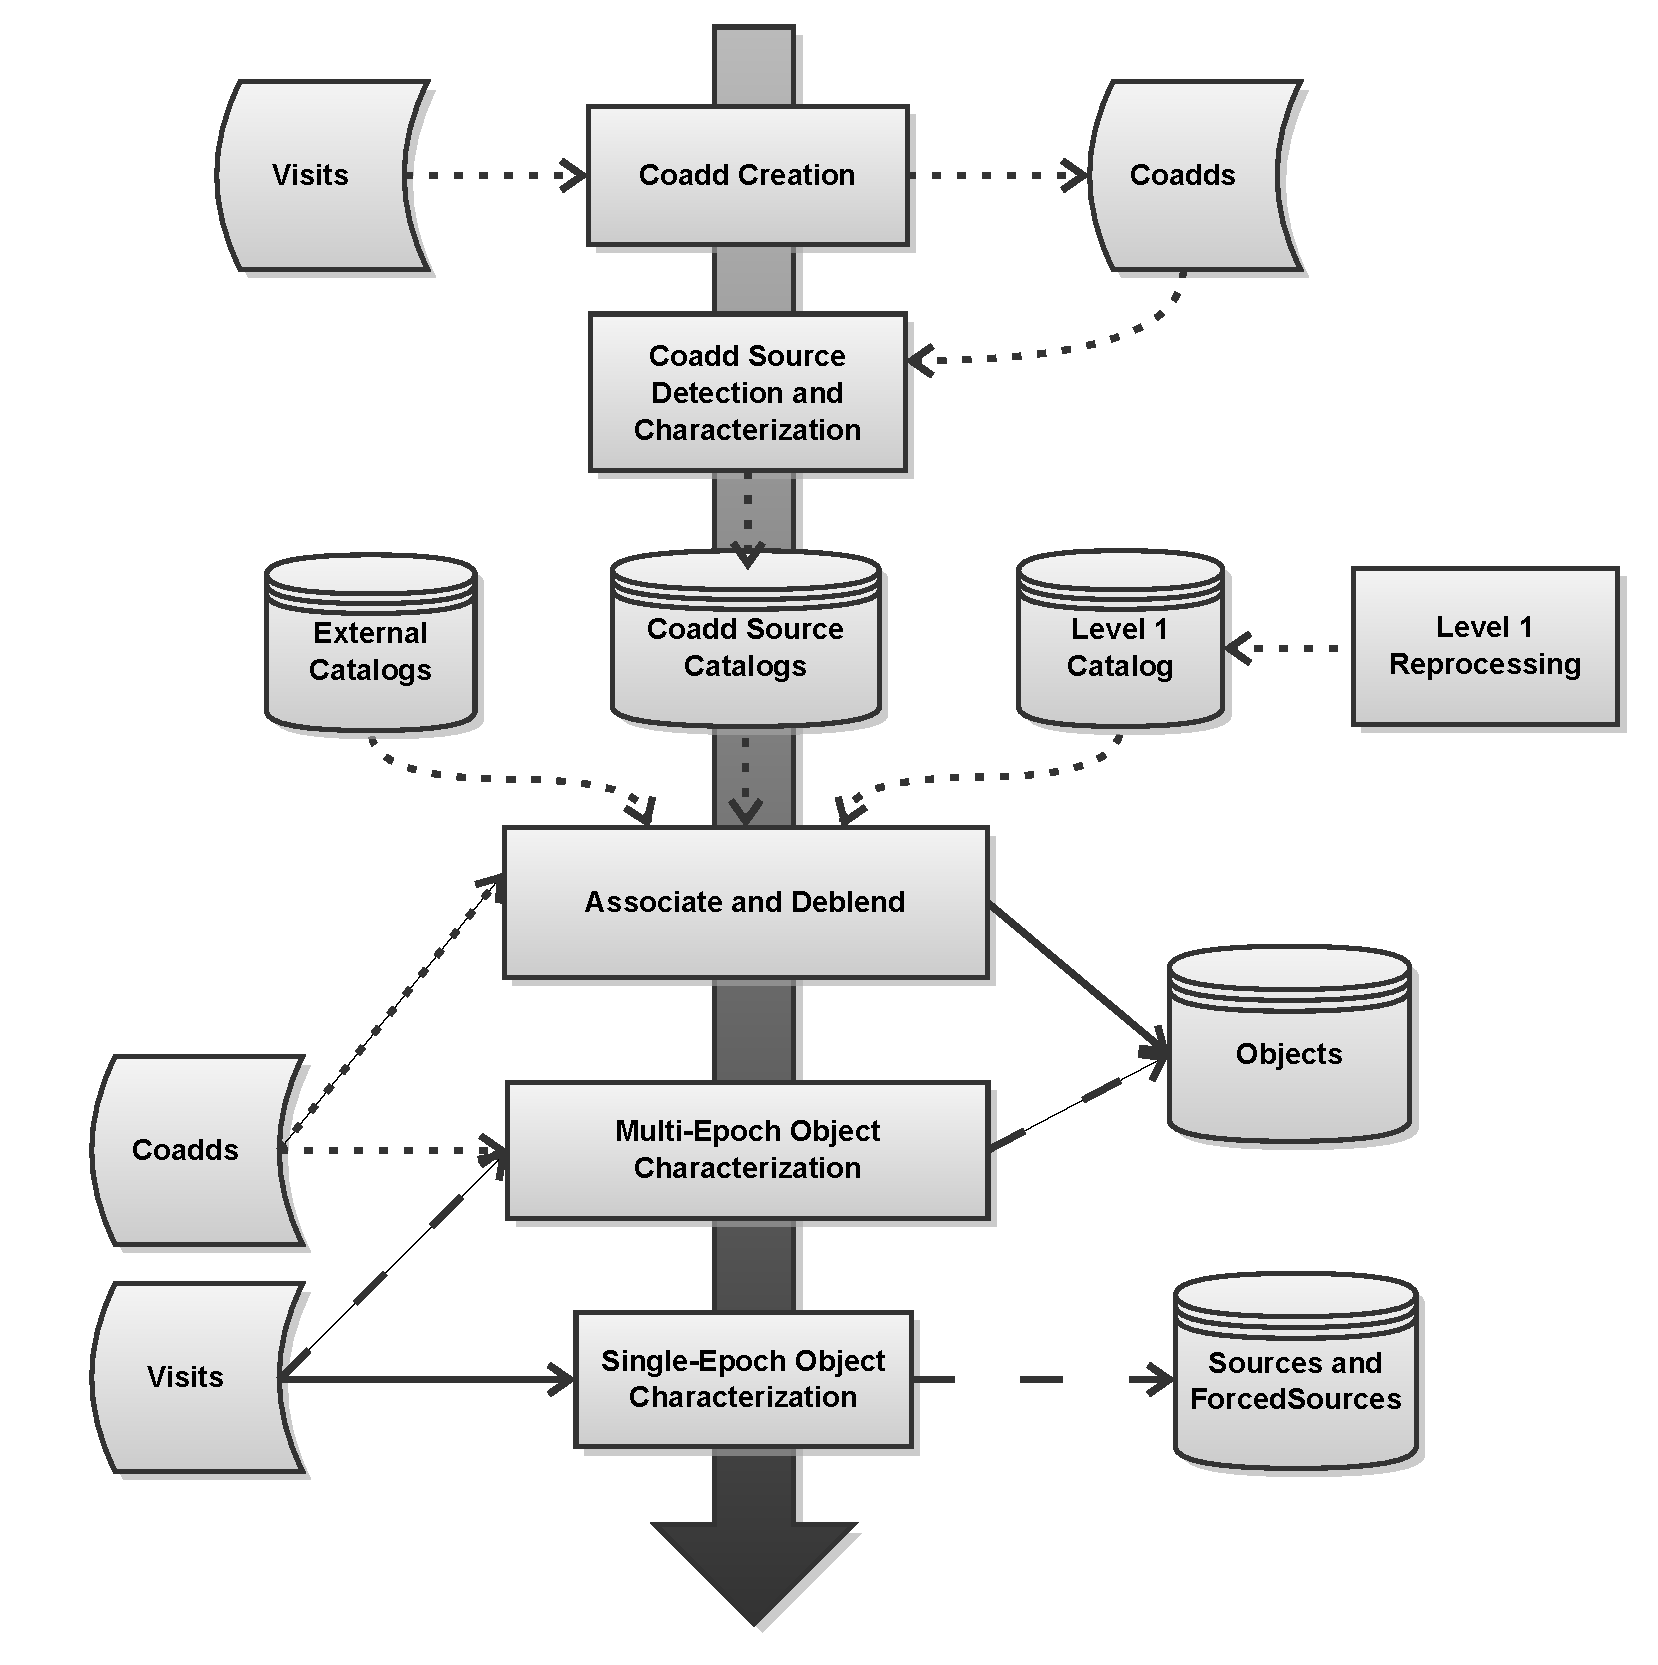
\includegraphics[scale=0.5]{Level_2_Processing_Flowchart}
    \caption{Level 2 Data Processing Overview}    
\end{figure}

\subsection{The Level 2 Database}

\subsection{Level 2 Image Products}

\subsection{Open Issues}


\end{document}
